\section{Experimental Setup}
\label{sec:experimental_setup}

\subsection{Simulation Environment and Mixed-Traffic Calibration}
\label{sec:sim_env}
All experiments are conducted in SUMO~v1.12.0~\cite{lopez2018_sumo}, configured with
the sub-lane model at a lateral resolution of $0.4$~m. This choice is deliberate
rather than cosmetic: in motorcycle-dominant traffic the conventional one-vehicle-per-lane
abstraction is invalid, as powered two-wheelers continuously filter laterally and form
wide, deformable clusters that conventional car-following models cannot reproduce. The
sub-lane resolution restores the lateral degrees of freedom required to capture this
filtering behaviour, consistent with microscopic observations of motorcycle dynamics under
Vietnamese mixed-traffic conditions~\cite{vn_roundabout}.

The vehicle composition is a central calibration target. The motorcycle count share is set
to $73\%$, anchored to the $72.6\%$ motorcycle mode share reported for
Ngoc~\emph{et~al.}~\cite{ngoc2021_fivecities}; the remaining demand is allocated to
passenger cars ($17\%$), trucks ($7\%$), and buses ($3\%$) by vehicle class.
Ngoc~\emph{et~al.}~\cite{ngoc2021_fivecities} also reports motorcycle shares of $\approx 80$--$89\%$ for Hai~Phong, Da~Nang, Ho~Chi~Minh~City, and
Can~Tho, a range deliberately bracketed by the composition sweep of
Section~\ref{sec:generalization}. We distinguish count share from traffic \emph{load}: at a motorcycle
passenger-car-unit (PCU) equivalence of $\approx 0.29$~\cite{cao_sano_hanoi},
a $73\%$ motorcycle count corresponds to only about one-third of the total PCU-based load,
with the exact fraction depending on the heavy-vehicle PCU values. Accordingly, count share
is used when reasoning about lateral filtering, whereas PCU is used for capacity
arguments. To reproduce realistic motorcycle swarming, the sub-lane parameters are set to
\texttt{latAlignment=arbitrary} with a minimum lateral gap \texttt{minGapLat},
which allows roughly three to four motorcycles to share a standard $3.2$~m urban lane
alongside a passenger car.

Under this calibration, a queue-discharge experiment yields a raw per-lane discharge of
approximately $2450$~veh/h---well above a conventional car-lane saturation flow because
motorcycles filter and discharge several abreast within a single lane. At the calibrated
$73\%$ motorcycle share this corresponds to roughly $1500$~PCU/h per lane, characteristic of
the mixed-flow regime documented for Hanoi~\cite{cao_sano_hanoi}. As regional compositions vary, the $73\%$ value is treated
as a representative anchor rather than a universal constant, and the policy's robustness to
compositional shift is defended explicitly through the systematic motorcycle sweep
($\{50\%, 73\%, 90\%\}$) of Section~\ref{sec:generalization}.

\subsubsection{Signal-Timing Bounds}
The minimum green time is fixed at $15$~s (three decision intervals).
This ensures that an activated phase discharges a meaningful platoon and suppresses the high-frequency
phase flickering that otherwise traps wide motorcycle clusters within the intersection. The
maximum green time is fixed at $60$~s. This value is justified by a simulation-based
design-selection pilot on the $16$-junction N3 grid (seed~$42$, $100$k training steps),
evaluated on held-out demand. As reported in Table~\ref{tab:maxgreen_pilot}, the $60$~s
bound dominates a relaxed $90$~s bound across all primary metrics; in particular, the
$90$~s bound severely degrades the $95$th-percentile (P95) waiting time
(the selected $60$~s bound is $24.7\%$ lower), because excessively long green phases starve cross-phase
movements, conflicting directly with the anti-starvation objective of the reward
(Section~\ref{sec:reward}). The bounds are therefore adopted as a structural
choice applied uniformly to every learned and heuristic controller. We note that the
maximum green time additionally sets the scale of the \texttt{green\_timer\_norm} feature
($\text{timer}/\text{max\_green}$); it is thus a coupled observation/model parameter
prior to training and held identical across all arms, with the SUMO-actuated controller's
\texttt{maxDur} matched to $60$~s for fairness.

\begin{table}[t]
  \centering
  \caption{Maximum-green selection pilot (N3 grid, seed~$42$, $100$k steps, held-out
  evaluation). Lower is better; the selected bound is in bold. Evaluation is based on an early
  $100$k-step convergence pilot used to structurally set the signal-timing constraints prior
  to full training, not on the converged policy.}
  \label{tab:maxgreen_pilot}
  \vspace{-4mm}
  \begin{tabular}{lccc}
    \toprule
    \textbf{Max-green} & \textbf{Travel time (s)} & \textbf{Waiting (s)} & \textbf{P95 waiting (s)}\\
    \midrule
    \textbf{$60$~s (selected)} & \textbf{311.1} & \textbf{135.8} & \textbf{504}\\
    $90$~s                     & 367.0          & 173.6          & 669\\
    \midrule
    $\Delta$ ($60$ vs.\ $90$)  & $-15.2\%$      & $-21.8\%$      & $-24.7\%$\\
    \bottomrule
  \end{tabular}
\end{table}

\subsection{Networks and Demand}
\label{sec:networks}
The framework is evaluated on two synthetic but structurally sound topologies: a
signalized corridor (denoted N2; $1 \times 5$ junctions) and a signalized grid
(denoted N3; $4 \times 4$ junctions). All intersections are four-way with two lanes per approach. The two scales
jointly probe both arterial coordination (the corridor) and network-level interaction under
many simultaneously learning agents (the grid).

To stress-test the controllers under non-stationary load rather than a single operating
point, vehicle insertions over the $5400$~s episode are drawn from an inhomogeneous Poisson
process following a time-varying trapezoidal profile. The profile ramps from an off-peak lull
to a sustained demand peak, eases to an intermediate plateau, and tapers back, exercising the
controllers across loading, saturation, and unloading regimes. The exact mathematical
formulation and rate parameters are provided in Appendix~\ref{app:demand}.
\begin{figure}[t]
    \centering
    \begin{subfigure}{\columnwidth}
        \centering
        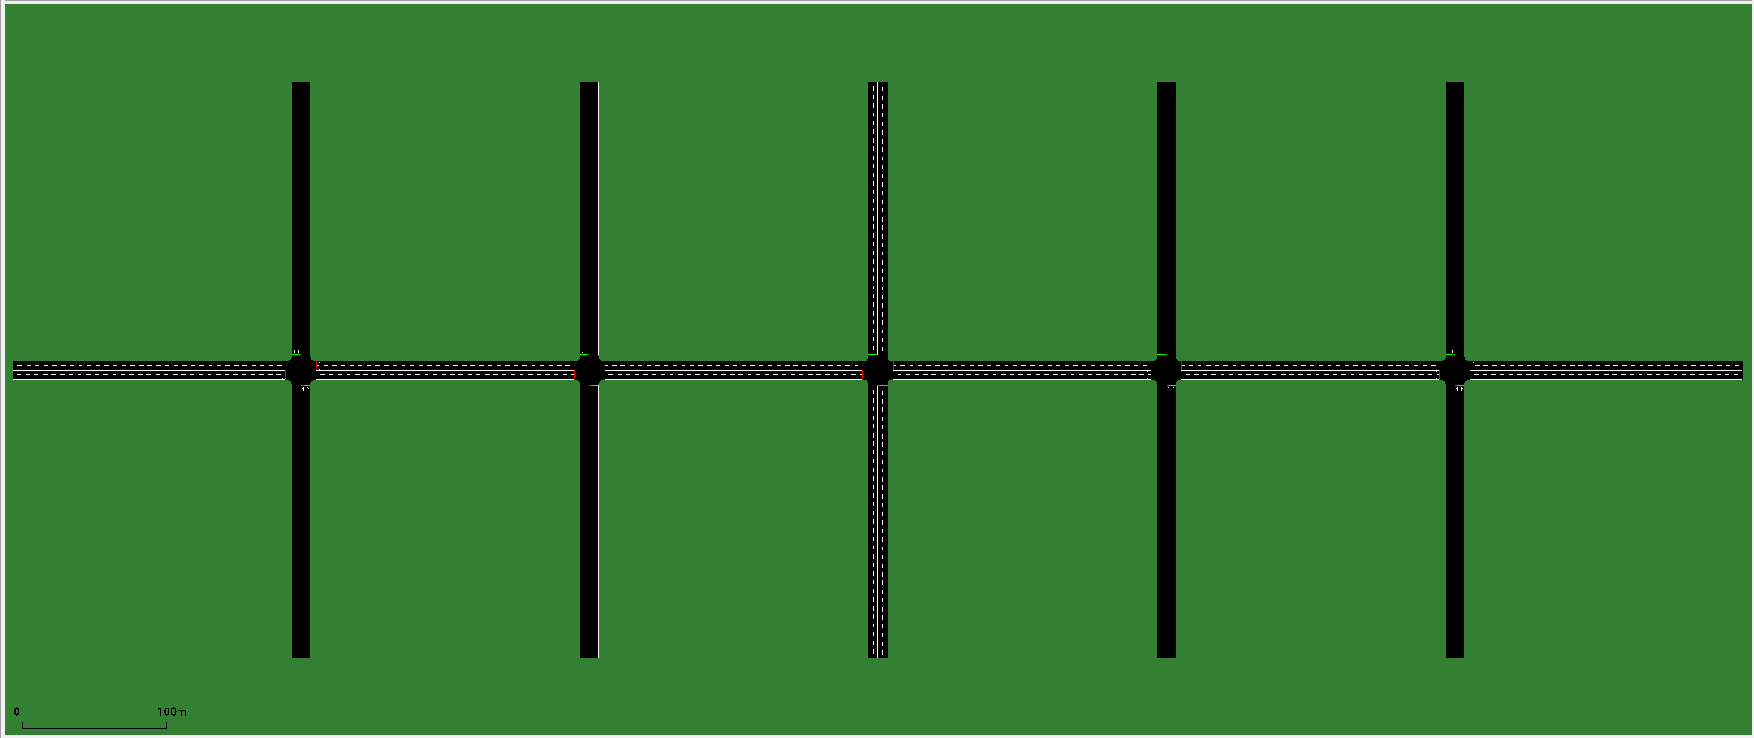
\includegraphics[width=\columnwidth]{assets/figures/n2_sumo.pdf}
        \caption{N2 corridor ($1\times5$, 5 intersections).}
        \label{fig:net_n2}
    \end{subfigure}
    \vspace{2mm}
    \begin{subfigure}{\columnwidth}
        \centering
        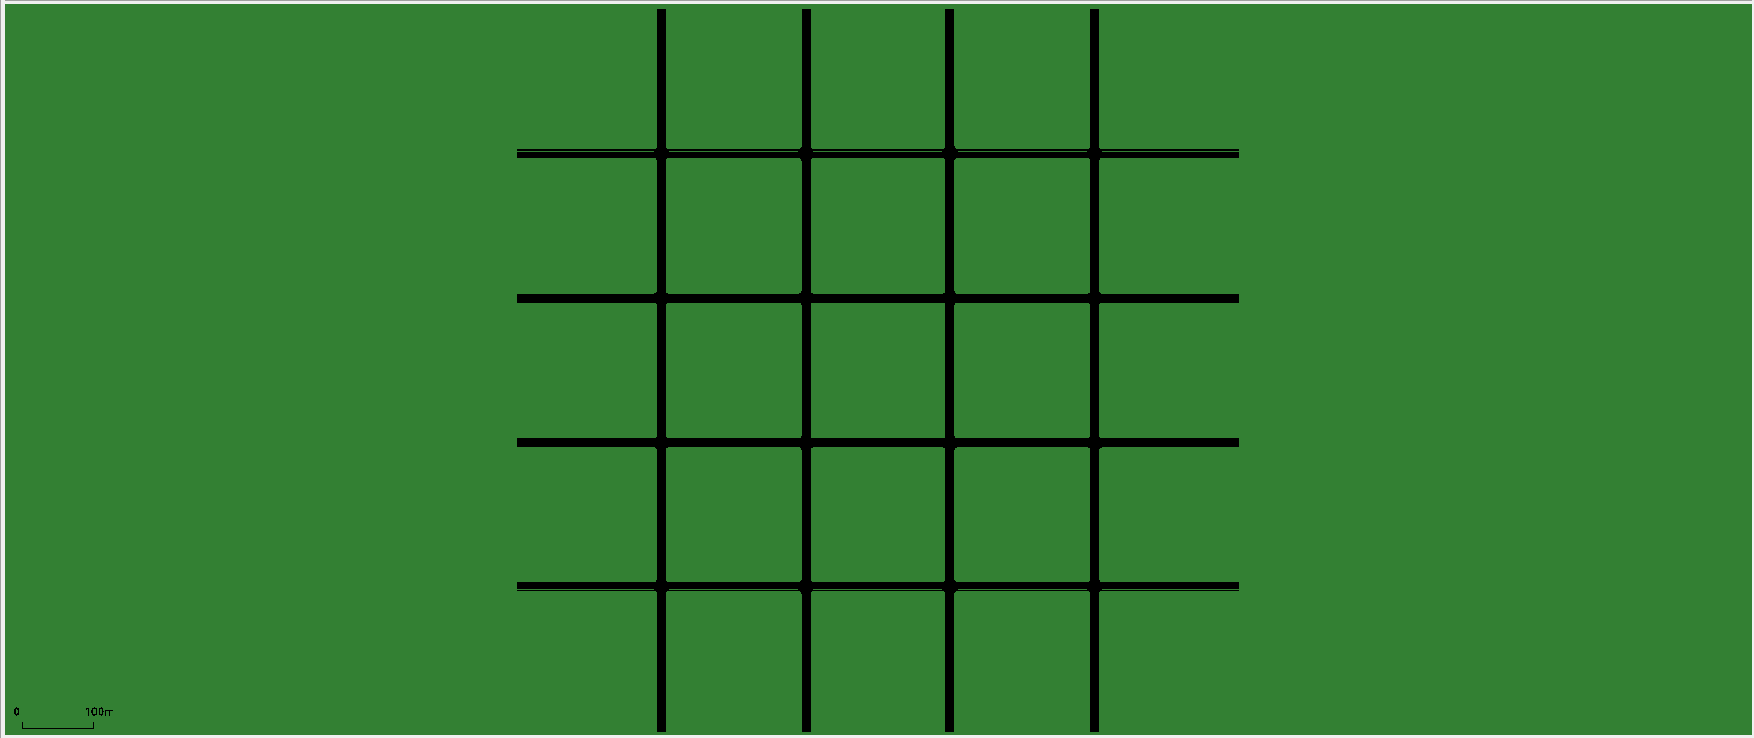
\includegraphics[width=\columnwidth]{assets/figures/n3_sumo.pdf}
        \caption{N3 grid ($4\times4$, 16 intersections).}
        \label{fig:net_n3}
    \end{subfigure}
    \caption{SUMO evaluation networks. All intersections are four-way with two lanes per approach; each intersection is controlled by one decentralized MAPPO agent.}
    \label{fig:networks}
    \vspace{-4mm}
\end{figure}
\subsection{Baselines}
\label{sec:baselines}
The proposed MAPPO controller is benchmarked against a spectrum of strong, non-strawman
baselines. To ensure a fair comparison, every heuristic is restricted to the same phase
groups, decision interval, and timing constraints as the learned policy.
\begin{itemize}
  \item \emph{Webster fixed-time}~\cite{webster1958}: an analytically derived fixed-time
        plan computed from PCU-weighted measured flows, with cycle length
        $C = (1.5L + 5)/(1 - Y)$ clamped to $[40, 120]$~s and proportional green splits.
        This provides a competitive classical baseline rather than a degenerate fixed-time
        plan. To ensure a strict and fair comparison, Webster's saturation flow is explicitly
        calibrated to the network's measured mixed-traffic sublane capacity
        ($\approx 1500$~PCU/h/lane), preventing artificial performance degradation that would
        occur if standard car-only saturation flows were assumed.
  \item \emph{SUMO-actuated}: the gap-based actuation controller native to
        SUMO~\cite{lopez2018_sumo}, configured with \texttt{minDur}~$=15$~s and
        \texttt{maxDur}~$=60$~s to match the learned controllers exactly.
  \item \emph{Max-Pressure}~\cite{varaiya2013_maxpressure}: a greedy pressure-based
        heuristic that consumes the identical observation pipeline and phase groups as the
        RL agents and grants right-of-way to the phase of highest pressure.
  \item \emph{IPPO}~\cite{dewitt2020_ippo}: an ablative learned baseline with an identical
        actor architecture and training budget but with independent per-agent critics
        conditioned solely on the local $26$-dimensional observation.
        This isolates the contribution of centralized training with decentralized execution.
  \item \emph{MAPPO-privileged (upper bound)}: the identical MAPPO~\cite{yu2022_mappo}
        algorithm whose observation is augmented to a $38$-dimensional vector incorporating
        exact, non-camera-observable simulator quantities (exact halting counts,
        waiting times, and total vehicle counts). The reward is held identical to the proxy
        arm and only the state visibility differs, so the gap between this arm and the proxy
        policy directly quantifies the \emph{information-restriction cost} of
        Section~\ref{sec:restriction_cost}.
\end{itemize}

\subsection{Metrics and Statistical Protocol}
\label{sec:metrics}
Performance is quantified by two primary metrics extracted from SUMO's \texttt{tripinfo}
output: mean travel time and mean waiting time. Secondary metrics comprise the P95 waiting
time (which captures starvation events masked by the mean), the throughput ratio, the mean
vehicle speed, and the number of phase switches per episode. Environmental indicators
(CO\textsubscript{2} emissions and fuel consumption, computed via the HBEFA-based emission
model~\cite{krajzewicz2015_emissions}) are evaluated post hoc and are never exposed to the
agent reward.

To ensure statistical rigour, each method is trained with five independent seeds
($42, 123, 456, 789, 1337$) and evaluated on ten held-out demand route-seeds per scenario.
All tabular results report the mean across training seeds together with a $95\%$ confidence
interval. Statistical significance is assessed against the strongest baseline using a
two-sided Mann--Whitney $U$ test~\cite{mann1947_mwu}, with $p$-values corrected for multiple
comparisons across scenarios by the Holm--Bonferroni procedure~\cite{holm1979}.
Effect size is reported through Cohen's~$d$~\cite{cohen1988} to guard against
statistically significant but negligible differences.

\subsection{Training Configuration and Reproducibility}
\label{sec:training}
Each model is trained to a fixed budget of $5 \times 10^{5}$ environment steps, a
horizon established by convergence pilots. Observation statistics are normalized by
Welford's algorithm~\cite{welford1962} and serialized into the checkpoint, so that
evaluation and deployment apply identical normalization without recompilation. The complete
set of MAPPO training hyperparameters---including PPO clip ratios, GAE discount factors, and
learning rates---is detailed in Appendix~\ref{app:hyperparams}.

To guarantee end-to-end reproducibility, the full codebase, trained checkpoints,
demand generators (\texttt{.rou.xml}), phase-group derivations, and evaluation scripts are
released publicly at \mbox{[REPOSITORY~URL]} under a tagged commit. The precise observation
and reward schema version is stamped into every run configuration, ensuring that all
results are traceable to an exact environment specification.

% [Hyperparameter table relocated to Appendix~\ref{app:hyperparams} (sec9_appendices.tex)]
